% Tekijä:   Teemu Likonen <tlikonen@iki.fi>
% Lisenssi: Creative Commons Nimeä-JaaSamoin 4.0 Kansainvälinen (CC BY-SA 4.0)
%           https://creativecommons.org/licenses/by-sa/4.0/legalcode.fi

\leijukuva{
  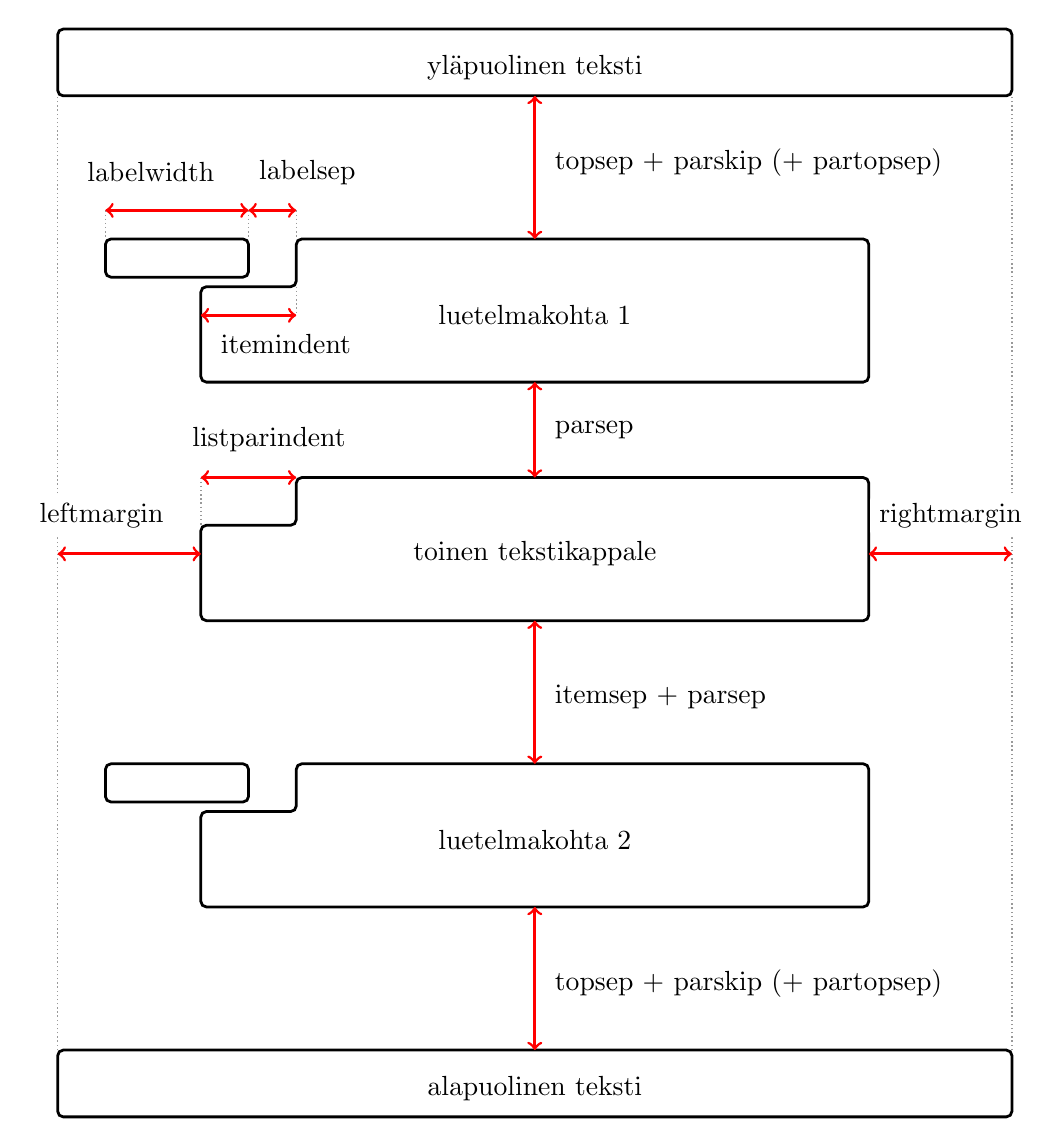
\begin{tikzpicture}
    [x=.01\textwidth, y=.01\textwidth, line width=1bp, rounded corners=2bp]

    \newcommand{\kpl}[1]{\draw (15,#1) -- ++(70,0) -- ++(0,15)
      -- ++(-60,0) -- ++(0,-5) -- ++(-10,0) -- cycle}
    \newcommand{\nuoli}[2]{\draw [color=red, <->] (#1) -- (#2)}
    \newcommand{\kyltti}[2]{\draw (#1) node [anchor=west, fill=white,
      baseline=0bp] {#2}}

    \newcommand{\katko}[2]{\draw [color=black!40, densely dotted, line
      width=.5bp] (#1) -- (#2)}

    \katko{0,10}{0,110};
    \katko{100,10}{100,110};

    \kpl{80};
    \kpl{55};
    \kpl{25};

    \draw (0,10) rectangle ++(100,-7);
    \node at (50,6) {alapuolinen teksti};

    \draw (0,110) rectangle ++(100,7);
    \node at (50,113) {yläpuolinen teksti};

    \nuoli{50,110}{50,95};
    \kyltti{51,103}{\mitta{topsep} + \mitta{parskip} (+ \mitta{partopsep})};

    % Ylin kappale
    \node at (50,87) {luetelmakohta 1};
    \draw (5,91) rectangle ++(15,4);
    \katko{5,98}{5,95};
    \katko{20,98}{20,95};
    \katko{25,98}{25,95};
    \nuoli{5,98}{20,98}; \kyltti{2,102}{\mitta{labelwidth}};
    \nuoli{20,98}{25,98}; \kyltti{20,102}{\mitta{labelsep}};
    \katko{25,90}{25,87};
    \nuoli{15,87}{25,87}; \kyltti{16,84}{\mitta{itemindent}};

    \nuoli{50,70}{50,80};
    \kyltti{51,75}{\mitta{parsep}};

    % Keskimmäinen kappale
    \node at (50,62) {toinen tekstikappale};
    \nuoli{0,62}{15,62};
    \kyltti{-3,66}{\mitta{leftmargin}};
    \nuoli{85,62}{100,62};
    \kyltti{85,66}{\mitta{rightmargin}};
    \katko{15,70}{15,65};
    \nuoli{15,70}{25,70};
    \kyltti{13,74}{\mitta{listparindent}};

    \nuoli{50,40}{50,55};
    \kyltti{51,47}{\mitta{itemsep} + \mitta{parsep}};

    % Alin kappale
    \node at (50,32) {luetelmakohta 2};
    \draw (5,36) rectangle ++(15,4);

    \nuoli{50,25}{50,10};
    \kyltti{51,17}{\mitta{topsep} + \mitta{parskip} (+ \mitta{partopsep})};
\end{tikzpicture}
}{
  \caption{Luetelmien tekemiseen tarkoitetun \ymparisto{list}\-/
    ympäristön mitat}
  \label{kuva:list-mitat}
}
